\documentclass[reqno]{amsart}

\usepackage[margin=2.5cm]{geometry}
\usepackage[pdftex]{graphicx}
\usepackage[utf8]{inputenc}
\usepackage[T1]{fontenc}
\usepackage{textcomp}
\usepackage{babel}
\usepackage{amsmath, amssymb, amsthm, amscd}
\usepackage[colorlinks=true,linkcolor=blue]{hyperref}
\usepackage{float}
\usepackage{mathrsfs}
%\usepackage{enumitem}
%% for identity function 1:
\usepackage{bbm}
%%For category theory diagrams:
\usepackage{tikz-cd}
%%For code (e.g. python) in latex:
%\usepackage{listings}
%
%Usage: 
%\begin{lstlisting}[language=Python]
%\end{lstlisting}

\newcommand{\incfig}[2][1]{%
\def\svgwidth{#1\columnwidth}
\import{./figures/}{#2.pdf_tex}
}


\theoremstyle{plain}% default
\newtheorem{theorem}{Theorem}[section]
\newtheorem{lemma}[theorem]{Lemma}
\newtheorem{proposition}[theorem]{Proposition}
\newtheorem{corollary}[theorem]{Corollary}


\theoremstyle{definition}
\newtheorem{definition}[theorem]{Definition}
\newtheorem{example}[theorem]{Example}
\newtheorem{exercise}[theorem]{Exercise}
\newtheorem{problem}[theorem]{Problem}


\theoremstyle{remark}
\newtheorem*{remark}{Remark}
\newtheorem*{note}{Note}
\newtheorem*{solution}{Solution}






% figure support
\usepackage{import}
\usepackage{xifthen}
\pdfminorversion=7
\usepackage{pdfpages}
\usepackage{transparent}

\pdfsuppresswarningpagegroup=1

\setlength\parindent{0pt}

\newcommand{\qedwhite}{\hfill \ensuremath{\Box}}

%Inequalities
\newcommand{\cycsum}{\sum_{\mathrm{cyc}}}
\newcommand{\symsum}{\sum_{\mathrm{sym}}}
\newcommand{\cycprod}{\prod_{\mathrm{cyc}}}
\newcommand{\symprod}{\prod_{\mathrm{sym}}}

%Linear Algebra

\DeclareMathOperator{\Span}{span}
\DeclareMathOperator{\Ima}{Im}
\DeclareMathOperator{\diag}{diag}
\DeclareMathOperator{\Ker}{Ker}
\DeclareMathOperator{\ob}{ob}
\DeclareMathOperator{\sk}{sk}
\DeclareMathOperator{\Vect}{Vect}
\DeclareMathOperator{\Set}{Set}
\DeclareMathOperator{\Group}{Group}
\DeclareMathOperator{\Ring}{Ring}
\DeclareMathOperator{\Ab}{Ab}
\DeclareMathOperator{\Top}{Top}
\DeclareMathOperator{\hTop}{hTop}
\DeclareMathOperator{\Htpy}{Htpy}
\DeclareMathOperator{\Cat}{Cat}
\DeclareMathOperator{\CAT}{CAT}
\DeclareMathOperator{\Cone}{Cone}
\DeclareMathOperator{\dom}{dom}
\DeclareMathOperator{\cod}{cod}
\DeclareMathOperator{\Aut}{Aut}
\DeclareMathOperator{\Mat}{Mat}
\DeclareMathOperator{\Fin}{Fin}
\DeclareMathOperator{\rel}{rel}
\DeclareMathOperator{\Int}{Int}
\DeclareMathOperator{\sgn}{sgn}
\newcommand{\SL}{{\mathrm{SL}}}
\newcommand{\mobgp}{{\mathrm{PSL}_2(\mathbb{C})}}
\newcommand{\Hom}{{\mathrm{Hom}}}
\newcommand{\id}{{\mathrm{id}}}
\newcommand{\Mod}{{\mathrm{Mod}}}
\newcommand{\ud}{{\mathrm{d}}}
\newcommand{\Vol}{{\mathrm{Vol}}}
\newcommand{\Area}{{\mathrm{Area}}}
\newcommand{\diam}{{\mathrm{diam}}}

\newcommand{\reg}{{\mathtt{reg}}}
\newcommand{\geo}{{\mathtt{geo}}}

\newcommand{\tori}{{\mathcal{T}}}
\newcommand{\cpn}{{\mathtt{c}}}
\newcommand{\pat}{{\mathtt{p}}}


%Row operations
\newcommand{\elem}[1]{% elementary operations
\xrightarrow{\substack{#1}}%
}

\newcommand{\lelem}[1]{% elementary operations (left alignment)
\xrightarrow{\begin{subarray}{l}#1\end{subarray}}%
}

%SS
\DeclareMathOperator{\supp}{supp}
\DeclareMathOperator{\Var}{Var}

%NT
\DeclareMathOperator{\ord}{ord}

%Alg
\DeclareMathOperator{\Rad}{Rad}
\DeclareMathOperator{\Jac}{Jac}

\DeclareMathAlphabet{\pazocal}{OMS}{zplm}{m}{n}
\newcommand{\unif}{\pazocal{U}}

\begin{document}

\section{Topological groups}

\begin{theorem}[]
    Every topological group is completely regular.
\end{theorem}

\begin{proof}
    a
\end{proof}

\section{Local Compactness}


\begin{proposition}[]
    Every locally compact Hausdorff space is completely regular ($T_{3
    \frac{1}{2}}$ ).
\end{proposition}

\begin{proof}
    Idea: a locally compact Hausdorff space is homeomorphic to an
    open subset of its one-point compactification which is
    a compact Hausdorff space and thus of a normal space.
\end{proof}


\section{Separation axioms}
\subsection{Urysohn Lemma}

\begin{theorem}[Urysohn Lemma]
    Let $X$ be a normal space; let $A$ and $B$ be disjoint closed subsets of
    $X$. Let $\left[ a,b \right] $ be a closed interval in the real line. Then
    there exists a continuous map
     \[
    f  \colon X \to \left[ a,b \right] 
    \] 
    such that $f(A) = \left\{ a \right\} $ and
    $f\left( B \right) = \left\{ b \right\} $.
\end{theorem}


\subsection{Strong Urysohn}

\begin{definition}[$G_{\delta} $ set]
    A set $A \subset X$ is a $G_{\delta}$ set in $X$ if 
    $A$ is the intersection of a countable collection of
    open sets of $X$.
\end{definition}

\begin{theorem}[]
    Let $X$ be normal. There exists a continuous function
    $f  \colon X \to \left[ 0,1 \right] $ such that
    $f(x) = 0$ for $x \in A$, and $f(x) >0$ for
    $x \not\in A$, if and only if $A$ is a closed
    $G_{\delta}$ set in $X$.\\
    A function satisfying the requirements of this theorem is
    said to \textbf{vanish precisely on $A$}.
\end{theorem}

\begin{proof}
    The idea is to use the standard idea of the Urysohn lemma:
    namely, constructing sets $U_p$ for all $p \in Q$ and
    defining a continuous function in $\left[ 0,1 \right] $ from these.\\
    Suppose $A = \bigcap_{i \in \cap } V_i$ where
    $V_i$ are open. If necessary, we can redefine
    $V_i' = \bigcap_{j=1}^{i} V_i$ so that
    $V_1' \supset V_2' \supset V_3' \supset \ldots$, so assume
    $V_1 \supset V_2 \supset \ldots$.
    Now let $U_1 = V_1$. Suppose $U_{\frac{1}{k}}$ is defined for
    $1 \le k \le  n$. By normality, we can find an open set
    $U_{\frac{1}{n+1}}$ such that
    $A \subset U_{\frac{1}{n+1}} \subset \overline{U_{\frac{1}{n+1}}}
    \subset U_{n} \cap V_n$.
    In this way we define sets $U_p$ for $p \in \left\{ \frac{1}{n}  \mid 
    n \in \mathbb{N} \right\} $. Suppose we have defined
$U_p$ for all $p \in P \subset \mathbb{Q} \cap (1, 0]$ where
$\left\{ \frac{1}{n} \mid n \in \mathbb{N} \right\} \subset P$. Choose
$p \in \left( \mathbb{Q} \cap (1,0] \right) - P$ and suppose
$a < p < b$ where $a,b \in P$, the by normality we can find an open set $U_p$
such that
$\overline{U_a} \subset U_p \subset \overline{U_p} \subset U_b$. In this way we
define $U_p$ for all $p \in \mathbb{Q} \cap (0,1]$. Now define
$U_0 = A$. Define 
$U_p = \varnothing$ for $p < 0$ and $U_p = X$ for $p > 1$. Define
$\mathbb{Q} (x) = \left\{ p  \mid x \in U_p \right\}  $ and
$f (x) = \inf \mathbb{Q}(x)$. Clearly if $x \in A$ then
$f(x) = 0$. If $x \not\in  A$ then there exists $N$ such that for all
$i \ge N$, we have $x \not\in V_i$. Hence for all $q \in [0, \frac{1}{N+1}) \cap
\mathbb{Q}$,
$x \not\in  U_{q}$, so $\inf \mathbb{Q}(x) \ge \frac{1}{N+1} > 0$, hence
$f(x) > 0$ as desired. Now to prove continuity: let $x_0 \in X$ and
$f(x_0) \in  (c,d)$. Choose numbers $p,q$ such that
$c < p < f(x_0) < q < d$. Then $U_q - \overline{U_p}$ is an open neighborhood
of $x_0$, and if $x \in U_q - \overline{U_p}$ then
$x \in U_q \subset \overline{U_q}$ so $f(x) \le q$ and since
$x \not\in  \overline{U_p}$, $x \not\in  U_p$ so $f(x) \ge p$. Thus
$f(x) \in \left[ p,q \right] \subset (c,d)$. Thus $f$ is continuous.
\end{proof}

\begin{theorem}[Strong Urysohn lemma]
    Let $X$ be a normal space. There is a continuous function $f  \colon X \to 
    \left[ 0,1 \right] $ such that $f(x) = 0$ for $x \in A$, and
    $f(x) = 1$ for $x \in B$, and $0 < f(x) < 1$ otherwise, if and only if
    $A$ and $B$ are disjoint closed $G_{\delta}$ sets in $X$.
\end{theorem}

\begin{proof}
    By the preceding theorem, we can find maps
    $f_1  \colon X \to \left[ 0,1 \right] $ such that
    $f_1 (A) = \left\{ 0 \right\} $ and
    $f_1 \left( X-A \right) \subset (0,1]$ and
    $g_2  \colon X \to \left[ 0,1 \right] $ such that
    $g_2 (B) = \left\{ 0 \right\} $ and
    $g_2 \left( X-B \right)  \subset (0,1]$. Now defining
    $f_2 (x) = 1-g_2(x)$ we find that
    $f_2 (B) = \left\{ 1 \right\} $ and
    $f_2 \left( X-B \right) \subset [0,1)$.
    \[
    h(x) = \frac{f_1(x)}{f_1(x) + g_2(x)}
    \] 
    satisfies the desired properties.
\end{proof}


\subsection{Tietze Extension Theorem}

\begin{theorem}[Tietze extension theorem]
    Let $X$ be a normal space; let $A$ be a closed subspace of $X$.
    \begin{enumerate}
        \item Any continuous map $A \to \left[ a,b \right] \subset \mathbb{R}$ 
            may be extended to a continuous map
            $X \to \left[ a,b \right] $.
        \item Any continuous map $A \to \mathbb{R}$ may be extended
            to a continuous map $X \to \mathbb{R}$.
    \end{enumerate}
\end{theorem}

\begin{remark}[]
    Suppose $A,B \subset X$ are closed disjoint subsets and $X$ is normal. Then
    define a map $f  \colon A \cup B \to \left[ 0,1 \right] $ by
    $f(A) = \left\{ 0 \right\} $ and $f(B) = \left\{ 1 \right\} $ where
    $A \cup B$ is in the subspace topology. This is well-defined as
    $A$ and $B$ are disjoint, and it is continuous since if
    $C \subset \left[ 0,1 \right] $ is a closed set, its preimage under
    $f$ is either empty or $A$ or $B$ or $A \cup B$, all of which are closed.
\end{remark}

\begin{exercise}[Munkres, 35.3]
    Let $X$ be metrizable. Show that the following are equivalent:
    \begin{enumerate}
        \item $X$ is bounded under every metric that gives the
            topology of $X$.
        \item Every continuous function $\varphi  \colon X \to \mathbb{R}$ 
            is bounded.
        \item $X$ is limit point compact.
    \end{enumerate}
\end{exercise}

\begin{proof}
    $(i) \implies (ii)$ : Suppose for any metric  $d$ giving the
    topology of $X$, $d(x,y) \le M_d$ for all $x,y \in X$.
    Now let $\varphi  \colon X \to \mathbb{R}$ be continuous. The map
    $X \to X \times \mathbb{R}$ by $x \mapsto x \times \varphi(x)$ is an embedding.
    Define a metric $\mu  \colon X \times X \to \mathbb{R}$ by
    $\mu (x,y) = d(x,y) + |\varphi(x) - \varphi(y)|$. Then
    clearly $\mu \ge 0$ with
    $\mu(x,y) = 0$ if and only if $x=y$. Clearly, $\mu(x,y) = \mu(y,x)$. Further,
    \[
    \mu(x,y) \le d(x,z) + d(z,y) +
    \left| \varphi(x) - \varphi(z) \right| + \left| \varphi(z) -
    \varphi(y)\right| 
    = \mu(x,z) + \mu(z,y).
    \] 
    Hence $\mu$ is indeed a metric.
    Now, suppose we take an $\varepsilon$-ball $B_{d}\left( x,\varepsilon \right) $ 
    in $X$ with the metric $d$, so
    $B_{d}(x,\varepsilon) = 
    \left\{ y \in X  \mid d(x,y) < \varepsilon \right\} $. Since
     \[
    d(x,z) \le d(x,z) + \left| \varphi(x) - \varphi(z) \right| =
    \mu (x,z)
    \] 
    we have
    $B_{\mu} (x, \varepsilon) \subset  B_d (x,\varepsilon)$.
    Let $B = \varphi^{-1}\left( B(\varphi(x), \frac{\varepsilon}{2}) \right) $.
    Since $d$ induces the topology on $X$, we can choose
    $\delta' < \frac{\varepsilon}{2}$ such that
    $B_d (x, \delta') \subset B$. Then for $z \in B_d \left( x, \delta' \right)
    $, we have
    \[
    \mu (x,z) = d(x,z) + \left| \varphi(x) - \varphi(z) \right| 
    < \delta' + \frac{\varepsilon}{2} < \varepsilon;
    \] 
    hence $B_d \left( x, \delta' \right) \subset 
    B_{\mu} \left( x, \varepsilon \right) $. Thus $\mu$ induces the same
    topology on $X$ as $d$, so $X$ is bounded under $\mu$. But then there
    exists $N$ such that
    $\mu \left( x,y \right) \le N$ for all $x,y \in X$. Then
    since $d (x,y) \le M_d$ for all $x,y \in X$, we have
    $\left| \varphi(x) - \varphi(y) \right| \le N - M_d$ for all
    $x,y \in X$, so $\varphi$ is bounded.\\
    \linebreak
    $(2) \implies (3)$ : Now, suppose every continuous function $\varphi  \colon
    X \to \mathbb{R}$
     is bounded.
     Suppose $A$ has an infinite set of points which has no limit points.
     Then $\overline{A} = A$, so $A$ is closed.
     Take some sequence $\left( x_i \right)_{i \in \mathbb{Z}_+}
     \subset A$. Similarly, $\left\{ x_i \right\}_{i \in \mathbb{Z}_+}$ is
     closed in $X$
     since it has no limit points in $X$. Define
     $f  \colon \left\{ x_i \right\}_{i \in \mathbb{Z}_+}\subset A \to \mathbb{R}$ by
     $f(x_i) = i$. Then
     if $\left( a,b \right) \subset \mathbb{R}$ with
     $\left( a,b \right) \cap \mathbb{Z}_+ = \left\{ 
     n, n+1, \ldots, n+k\right\} $, we have
     $f^{-1}\left( (a,b) \right) =
     \left\{ x_n, x_{n+1},\ldots, x_{n+k} \right\} $ which is open since
     each $\left\{ x_i \right\} $ is an open set: this is because since
     $A$ is not limit point compact, for each $x_i$, there exists
     a neighborhood $U_i$ such that $U_i \cap A = \left\{ x_i \right\} $.
     Thus $f$ is continuous and also $f$ is a surjection onto
     $\mathbb{Z}_+$.
     Now, since $X$ is a metric space and thus normal, and since
     $A$ is closed and $f$ is a map $\left\{ x_i \right\}_{i \in \mathbb{Z}_+}
     \to \mathbb{R}$, the Tietze extension
     theorem says that $f$ can be extended to a map
     $X \to \mathbb{R}$. However, also $f$ is unbounded since it
     is surjective on $\mathbb{Z}_+$, yet all continuous maps
     $X \to \mathbb{R}$ are bounded by assumption. Thus $A$ must contain
     some limit point, and hence $X$ is limit point compact.\\
     \linebreak
     $\left( 3 \right) \implies (1)$ : We show the contrapositive.
     Assume $X$ is not bounded under a metric $d$ inducing the topology on
     $X$.
     Let $x_0 \in X$. If
     there does not exist a point $y \in X$ such that
     $d(x_0,y) > N$ for some $N >0$ then for any two points
     $x,y \in X$ 
     \[
     d(x,y) \le d(x,x_0) + d(x_0,y) \le 2N,
     \] 
     so $X$ will be bounded. Hence we can
     choose a point $x_1 \in X$ such that
     $d_1 := d(x_0, x_1) > \varepsilon$. Then
      to define $d_n$, choose $x_n$ such that
      $d(x_0, x_n) > \varepsilon +  \sum_{i=0}^{n-1} d\left( x_i, x_{i+1} \right) $ and define
      $d_n := d\left( x_0, x_n \right) $. We claim that
      the set
      $\left\{ x_i \right\}_{i \in Z_0^{+}}$ is not limit point compact.
      Suppose first $x_n$ is a limit point. Then
      \[
      d(x_n, x_m) > d(x_n, x_{m-1}) - d\left( x_m, x_{m-1} \right) 
      > \ldots > d\left( x_n, x_{0} \right)  -
      \sum_{r = 0}^{m-1} d\left( x_{r+1}, x_{r} \right) 
      > \varepsilon
      \] 
      hence $B_{x_i, \frac{\varepsilon}{2}} \cap 
      \left\{ x_j \right\}_{j \in \mathbb{Z}_0^{+}} = \left\{ x_i \right\} $ 
      for all $i \in \mathbb{Z}_{0}^{+}$.\\
      Now suppose some $z \in X$ is a limit point. Then
      there exists $x_N$ such that
      $x_N \in B\left( z, \frac{\varepsilon}{2} \right) $. By normality, we can
      choose some $\delta$ with $\frac{\varepsilon}{2} > \delta > 0$ such that
      $x_N \not\in B\left( z, \delta \right) $, so $d\left( z,x_N \right) \ge 
      \delta$. Then for any  $M \neq N$
     \[
     d\left( z,x_M \right) \ge 
     d\left( x_M , x_N \right) - d\left( z, x_N \right) >
     \varepsilon - d\left( z, x_N \right)  > \frac{\varepsilon}{2} 
     > \delta
     \] 
     Hence $d\left( z, x_i \right) > \delta$ for all $i$, so
     $z$ is not a limit point as
     $B \left( z, \delta  \right) \cap 
     \left\{ x_j \right\}_{j \in \mathbb{Z}_0^{+}} = \varnothing$.
     Thus $\left\{ x_j \right\}_{j \in \mathbb{Z}_0^{+}}$ is an
     infinite subset of $X$ with no limit point in $X$, so
     $X$ is not limit point compact.
\end{proof}


\begin{exercise}[Munkres 35.4]
    Let $Z$ be a topological space. If $Y$ is a subspace of
    $Z$, we say that $Y$ is a \textbf{retract} of $Z$ if there
    is a continuous map $r  \colon Z \to Y$ such that
    $r(y) = y $ for each $y \in Y$.
    \begin{enumerate}
        \item Show that if $Z$ is Hausdorff and $Y$ is a retract of $Z$, then
            $Y$ is closed in $Z $.
        \item Let $A$ be a two-point set in $\mathbb{R}^2$. Show that
            $A$ is not a retract of $\mathbb{R}^2$.
        \item Let $S^{1}$ be the unit circle in $\mathbb{R}^2$ ; show that
            $S^{1}$ is a retract of $\mathbb{R}^2 - \left\{ 0 \right\} $.
    \end{enumerate}
\end{exercise}

\begin{proof}
    $(1)$ : Suppose $z$ is a limit point of $Y$ which is not in $Y$.
    Then all neighborhoods of $z$ intersect $Y$. 
    Since $z \neq r(z)$, we can take neighborhoods $U,V$ of
    $z$ and $r(z)$ respectively, such that
    $U \cap V = \varnothing$. Thus $U \not \subset \overline{V}$. Then
    $r^{-1}(V)- \overline{V}$ contains $z$ and thus intersects $Y$.
    Let $y \in r^{-1}(V) - \overline{V}$. Then
    $y = r(y) \in V \subset \overline{V}$, contradiction.
    Hence no such $z$ exists, so $Y$ contains all its limit points. Hence
    $Y$ is closed in $Z$.\\
    \linebreak
    $(2)$ : Suppose $r  \colon \mathbb{R}^2 \to A$ is a retract where
    $A = \left\{ x,y \right\} $. Then
    since $x,y$ are distinct and $\mathbb{R}^2$ is Hausdorff, $A$ is discrete,
    so
    $r^{-1}(x), r^{-1}(y)$ is a separation of $\mathbb{R}^2$. But
    $\mathbb{R}^2$ is connected. Contradiction. Hence $A$ is not a retract of
    $\mathbb{R}^2$. In fact, this reasoning shows that no finite subset
    of $\mathbb{R}^n$ with more than one point is a retraction of
    $\mathbb{R}^n$.\\
    \linebreak
    $(3)$ : Define $r  \colon \mathbb{R}^2 - \left\{ 0 \right\} \to S^{1}$ by
    $r(x) = \frac{x}{\|x\|}$. This is clearly a retraction.
\end{proof}

\begin{exercise}[35.5]
    A space $Y$ is said to have the \textbf{universal extension property} if
    for each triple consisting of a normal space $X$, a closed subset
    $A$ of $X$, and a continuous function $f  \colon A \to Y$, there
    exists an extension of $f$ to a continuous map of $X$ into
    $Y$.
    \begin{enumerate}
        \item Show that $\mathbb{R}^{J}$ has the universal extension
            property.
        \item Show that if $Y$ is homeomorphic to a retract of
            $\mathbb{R}^{J}$, then $Y$ has the universal extension
            property.
    \end{enumerate}
\end{exercise}

\begin{proof}
   $(1)$ : Firstly, the Tietze extension lemma thus says that
    $\mathbb{R}$ (as well as $[a,b]$ ) has the universal extension property.
    Now suppose we have a map $f  \colon A \to \mathbb{R}^{J}$. Then each
    component function $f_{\alpha}  \colon A \to \mathbb{R}$ is continuous
    and thus can be extended to a map $\tilde{f_{\alpha}}  \colon X \to
    \mathbb{R}$. Hence the map
    $\tilde{f}  \colon X \to \mathbb{R}^{J}$ defined by
    $\tilde{f}(x) = \left( \tilde{f_1}(x), \tilde{f_2}(x), \ldots \right) $ is 
    continuous and an extension of $f  \colon A \to \mathbb{R}^{J}$.\\
    \linebreak
    $(2)$ : Suppose $Y$ is a retract of $\mathbb{R}^{J} $ under
    $r  \colon \mathbb{R}^{J} \to Y$. Then $Y$ is closed in
    $\mathbb{R}^{J}$. Suppose $f  \colon
    A \to Y$ is a continuous map where $A$ is a closed subset of
    a normal space $X$.\\
    Then there are finitely many components $f_{\alpha_1}  \colon
    A \to Y_{\alpha_1},\ldots, f_{\alpha_n}  \colon A \to 
    Y_{\alpha_n}$ which we must extend, so it suffices to show that
    if $r  \colon \mathbb{R} \to Y$ is a retract then $Y$ has the universal
    extension property. Since $\mathbb{R}$ is path-connected, so is $Y$.
    As it is closed as well, $Y$ is an interval $\left[ a,b \right] $.
    But $\left[ a,b \right] $ has the universal extension property by
    the Tietze extension theorem, so
    $r$ can be extended, and thus $Y$ has the universal extension property. 
    If $\tilde{Y}$ is homeomorphic to $ Y$ under a homeomorphism
    $\varphi  \colon \tilde{Y} \to Y$ and we have a map
    $\tilde{f}  \colon A \to \tilde{Y}$, then
    $\varphi \circ \tilde{f}  \colon A \to Y$ is a continuous map and thus 
    has an extension onto all of  $X$, $\overline{\varphi \circ \tilde{f}} \colon
    X \to Y$, so in particular,
    $\varphi^{-1} \circ \overline{\varphi \circ \tilde{f}} \colon
    X \to \tilde{Y}$ is an extension of $\tilde{f}$ as it agrees with
    $\tilde{f}$ on $A$.
\end{proof}

\begin{exercise}[Munkres, 35.6]
    Let $Y$ be a normal space. Then $Y$ is said to be an \textbf{absolute
    retract} if for every pair of spaces $\left( Y_0, Z \right) $ such that
    $Z$ is normal and $Y_0$ is a closed subspace of $Z$ homeomorphic to $Y$,
    the space $Y_0$ is a retract of $Z$.
    \begin{enumerate}
        \item Show that if $Y$ has the universal extension property, then
            $Y$ is an absolute retract.
        \item Show that if $Y$ is an absolute retract and $Y$ is compact, then
            $Y$ has the universal extension property.
    \end{enumerate}
\end{exercise}

\begin{proof}
    $(a)$ : Suppose $Y$ is normal and we have a normal space
    $Z$ with a closed subspace $Y_0$ where $Y_0$ is homeomorphic to
    $Y$ under $\varphi  \colon Y_0 \to Y$. Suppose $Y$ has the universal
    extension property. Since $\varphi$ is continuous, it extends to
    a continuous map $\tilde{\varphi}  \colon Z \to Y$ which agrees with
    $\varphi$ on $Y_0$. Now
    $\varphi^{-1} \circ \tilde{\varphi}  \colon Z \to Y_0$ is a continuous map
    and on $Y_0$, $\tilde{\varphi}$ equals $\varphi$, so
    $\varphi^{-1} \circ \tilde{\varphi}$ is the identity on
    $Y_0$. Hence $\varphi^{-1} \circ \tilde{\varphi}$ is a retract
    of $Z$ onto $Y_0$.\\
    \linebreak
    $(b)$ : Since $Y$ is an absolute retract, it is normal and hence
    can be embedded into $\left[ 0,1 \right]^{J}$. Now, by Tychonoff's theorem, 
    $\left[ 0,1 \right]^{J}$ is compact. Now, the embedding of
    $Y$ is compact since $Y$ is compact, and since compact subspaces of
    Hausdorff spaces are closed, the embedding of $Y$ is a closed subspace.
    By the absolute retraction property, the embedding is a retract of
    $\left[ 0,1 \right]^{J}$ and by problem
    35.5, $Y$ thus has the universal extension property.
\end{proof}

\begin{exercise}[Munkres, 35.7]
    \begin{enumerate}
        \item Show that the logarithmic spiral
    \[
    C = \left\{ 0 \times 0 \right\} \cup
    \left\{ e^{t} \cos t \times  e^{t} \sin t  \mid  t \in \mathbb{R} \right\} 
    \] 
    is a retract of $\mathbb{R}^2$. Can you define a specific retraction
    $r  \colon \mathbb{R}^2 \to C$?
\item Show that the "knotted $x$-axis" $K$ of the figure is a retract of
    $\mathbb{R}^3$.
    \end{enumerate}
    \begin{figure}[H]
        \centering
        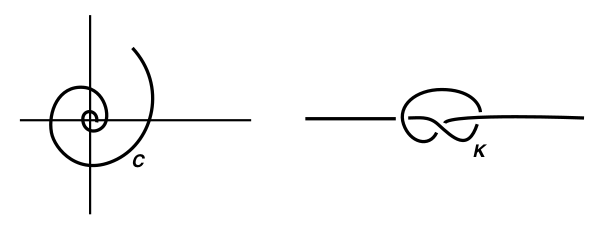
\includegraphics[width=0.5\textwidth]{retracts.png}
        \label{fig:retracts-png}
    \end{figure}
\end{exercise}


\begin{proof}
    $(a)$ : The spiral is homeomorphic with $\mathbb{R}$ by the hemeomorphism:
    \begin{align*}
        C &\to \mathbb{R}\\
        \left( x,y \right) &\mapsto \ln \left( \| (x,y) \| \right).
    \end{align*}
    Now, $\mathbb{R}$ has the universal extension property by problem
    35.5.(a), so by problem 35.6.(a), it is an absolute retract.
    Now, since $\mathbb{R}^2$ is normal and $C \subset \mathbb{R}^2$ is
    a closed subspace homeomorphic to $\mathbb{R}$, we find by the definition
    of an absolute retract that $C$ is a retract of $\mathbb{R}^2$.\\
    \linebreak
    Define now a map
    $r  \colon \mathbb{R}^2 \to C$ by
    \[
    r\left( x,y \right) = e^{ \ln \| (x,y)\|} \cos \left( \ln \|(x,y)\| \right)
    \times 
    e^{\ln \| (x,y) \|} \sin \left( \ln \|(x,y)\| \right) 
    \] 
    for $(x,y) \neq 0$ and
    $r\left( 0,0 \right) = (0,0)$. This is continuous as each component
    function is a composition of continuous functions which has limit $0$ as
    $(x,y) \to 0$. And it is clearly a retraction.\\
    \linebreak
    $(b)$ : This knotted $x$-axis is homeomorphic to the real line as well, so
    it has the universal extension property and is thus an absolute retract
    with the same reasoning as in part $(a)$ of this problem. The knot is
    clearly a closed subset of $\mathbb{R}^3$ and $\mathbb{R}^3$ is normal, so
    again we find that it is a retract of $\mathbb{R}^3$.
\end{proof}

\begin{theorem}[Munkres, exercise 35.8]
    Let $Y$ be a normal space. Then $Y$ is an absolute retract if and only
    if $Y$ has the universal extension property.
\end{theorem}

\begin{proof}
    One direction is exercise 35.6.(a).\\
    We must show that if $Y$ is an absolute retract, then $Y$ has the universal
    extension property. We will make use of the following proposition:

    \begin{proposition}[Adjunction spaces of normal spaces are normal]
    Suppose $X$ and $Y$ are disjoint normal spaces, $A$ is closed in $X$ and
    $f  \colon A \to Y$ is a continuous map.
    Then $Y \cup_f X$ is normal.
    \end{proposition}

    \begin{proof}
        Suppose $B,C \subset Y \cup_f X$ are closed disjoint subsets.
        Then $\pi^{-1}(B)$ and $\pi^{-1}(C)$ are disjoint closed subsets
        of $X \cup Y$ which is normal. \\
        Now, $\tilde{B} = \pi^{-1}(B) \cap Y$ and $\tilde{ C }= 
        \pi^{-1}(C) \cap Y$ are closed disjoint sets
        in $Y$, so as $Y$ is normal, we can separate them by a continuous
        function
        $g  \colon Y \to \left[ 0,1 \right] $ such that
        $g\left( \pi^{-1}(B) \cap Y \right) = \left\{ 0 \right\} $ and
        $g \left( \pi^{-1}(C) \cap Y \right) = \left\{ 1 \right\} $. Then
        $g \circ f  \colon A \to \left[ 0,1 \right] $ is a map such that
         $\pi^{-1}(B) \cap A \subset  \left( g \circ f \right)^{-1} \left( 0 \right) $
         and $\pi^{-1}(C) \cap A \subset 
         \left( g \circ f \right)^{-1} \left( 1 \right) $.
         Define a map $h  \colon A \cup Y \to \left[ 0,1 \right] $ by
         \[
         h(x) = \begin{cases}
             g \circ f (x),& x \in A\\
             g (x),& x \in Y
         \end{cases}
         \] 
         Then $h$ is continuous and separates
         $\pi^{-1}(B) \cap \left( A \cup Y \right) $ and
         $\pi^{-1}(C) \cap  \left( A \cup Y \right) $. 
         Now define $h \left( \pi^{-1}(B) \cap (X-A) \right) = \left\{ 0 \right\} $ 
         and $h \left( \pi^{-1}(C) \cap (X-A) \right) = \left\{ 1 \right\} $.
         Then
         $h$ is still continuous, and we can extend it to
         $X \cup Y$ by the Tietze extension lemma.
         Now $U = h^{-1}\left( [0,\frac{1}{2}) \right) $ and
         $V = h^{-1}\left( (\frac{1}{2},1] \right) $ are open disjoint sets
         around $\pi^{-1}(B)$ and $\pi^{-1}(C)$ respectively. Suppose
         $\left[ z \right] \in Y \cup_f X$. If $z' \in \left[ z \right] \cap
         Y$, then $h(z') = g(z')$. Now, if
         $z'' \in \left[ z \right] \cap A$, then
         $h(z'') = g\left( f(z'') \right) = g(z')$.
         Thus $h$ factors through $Y \cup_f X$, so
         \begin{equation*}
         \begin{tikzcd}
             Y \cup_f X  \ar[rd, "\tilde{h}"'] & X \cup Y \ar[d, "h"] \ar[l,
             "\pi"']\\
                               & \left[ 0,1 \right] 
         \end{tikzcd}
         \end{equation*}
         commutes. Now by the universal property of quotient maps and since
         $h = \tilde{h} \circ \pi$ is continuous, we have that
         $\tilde{h}$ is continuous, and
         $\tilde{h}^{-1}\left( [0, \frac{1}{2}) \right) $ and
         $\tilde{h}^{-1} \left( (\frac{1}{2},1] \right) $ are disjoint open sets
         around $B$ and $C$, respectively.
     \end{proof}
     Now suppose $X$ is a normal space and $A \subset X$ is a closed subset and
     $f  \colon A \to Y$ is continuous. Then we can form the
     adjunction space $Y \cup_f X$ which is normal by the above proposition.
     Since $Y \subset Y \cup_f X$ is homeomorphic with $Y$, and $Y$ is an
     absolute retract, we have that $Y \subset Y \cup_f X$ is a retract
     of $Y \cup_f X$. I.e., there exists a map $r  \colon
     Y \cup_f X \to Y$ such that $r \left( \left[ y \right]  \right) 
     = y$ for $\left[ y \right] \in Y \subset Y \cup_f X$. Now define
     $f  \colon X \to Y$ by
     \[
     f\left( x \right)  = i_Y^{-1} \circ r \circ i_X (x)
     \] 
     where $i_X  \colon X \to Y \cup_f X$ and
     $i_Y  \colon Y \to Y \cup_f X$ are the inclusions.
     Since $i_X$ and $i_Y$ are homeomorphisms and $r$ is continuous,
     $f$ is continuous and clearly agrees with the previous definition on
     $A$ since $r \circ i_X (a) = r \left( \left[ a \right]  \right) 
     = r \left( \left[ f(a) \right]  \right) 
     = \left[ f(a) \right] $ which maps to $f(a)$ by 
     $i_Y^{-1}$.
\end{proof}
     
     
    

    









%\bibliography{refs}
\end{document}
